\section{Ejemplo 5}

    \lipsum[1]

    \begin{figure}[h]
        \centering
        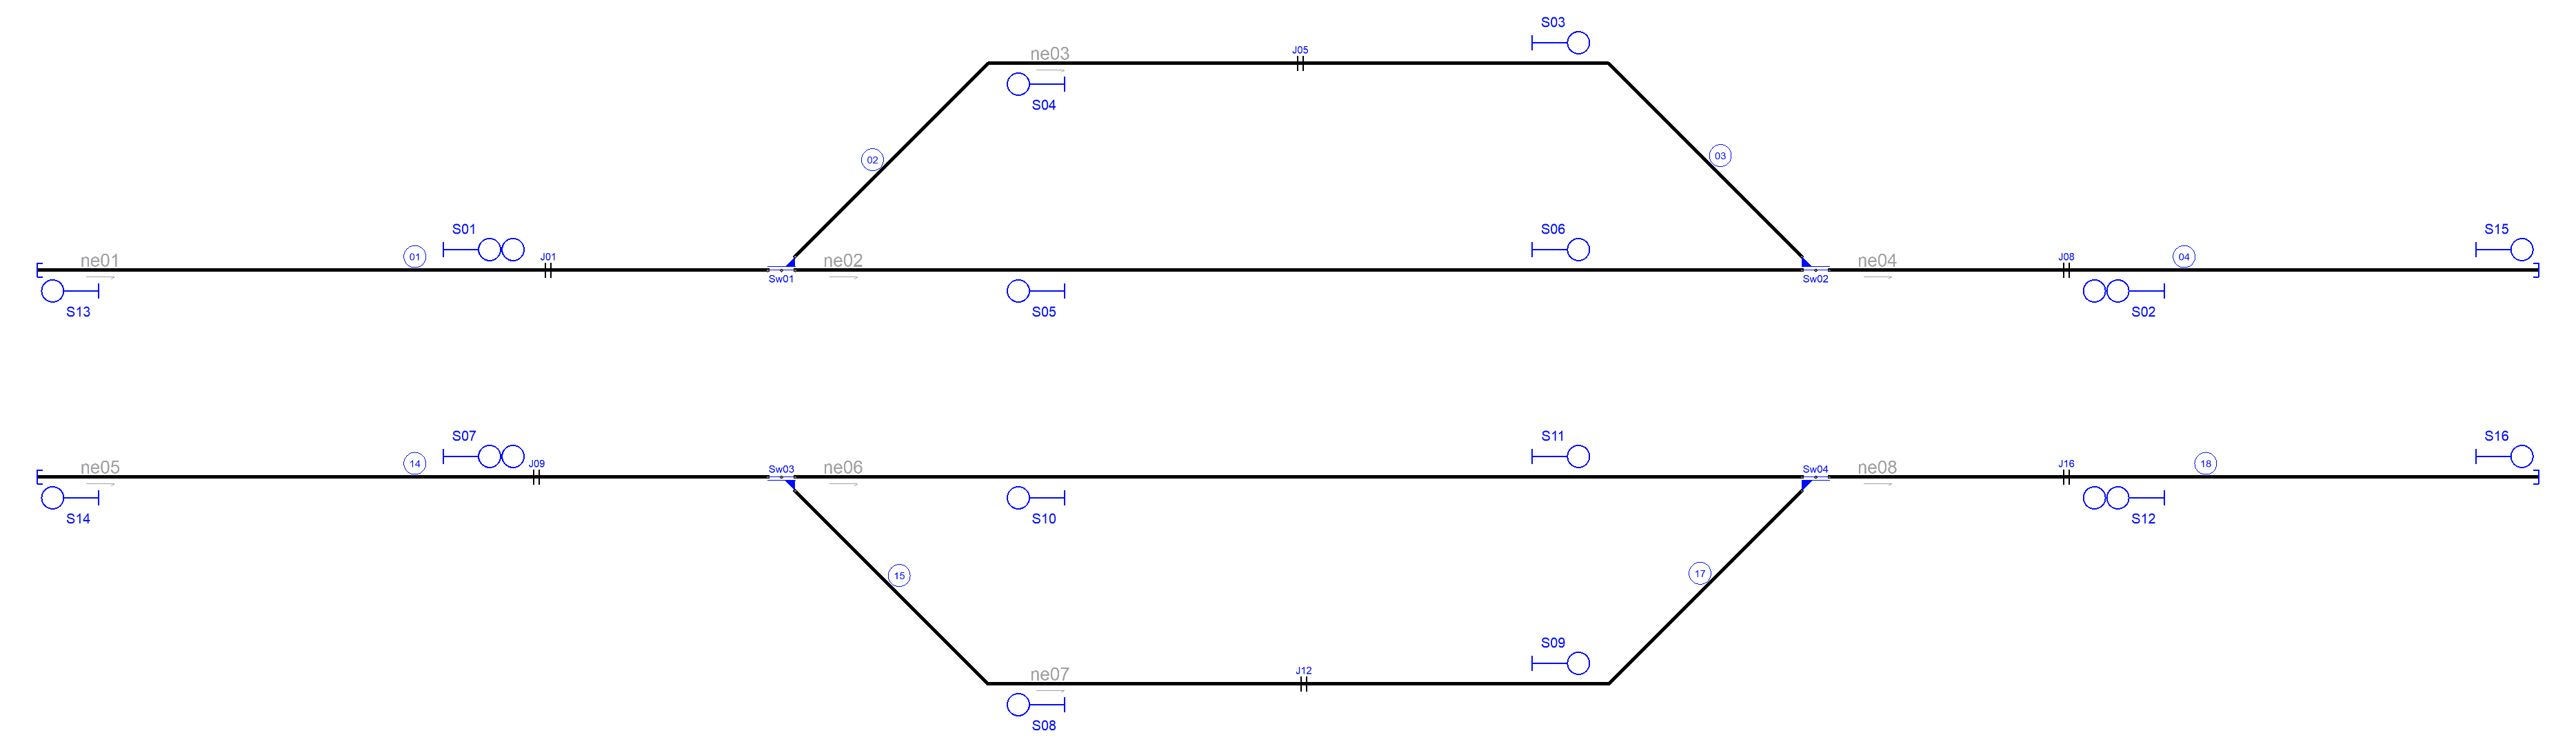
\includegraphics[width=1\textwidth]{resultados-obtenidos/ejemplo5/images/5_original.png}
        \centering\caption{Señalamiento original del ejemplo 5.}
        %\label{fig:LC_P2}
    \end{figure}

    \begin{figure}[h]
        \centering
        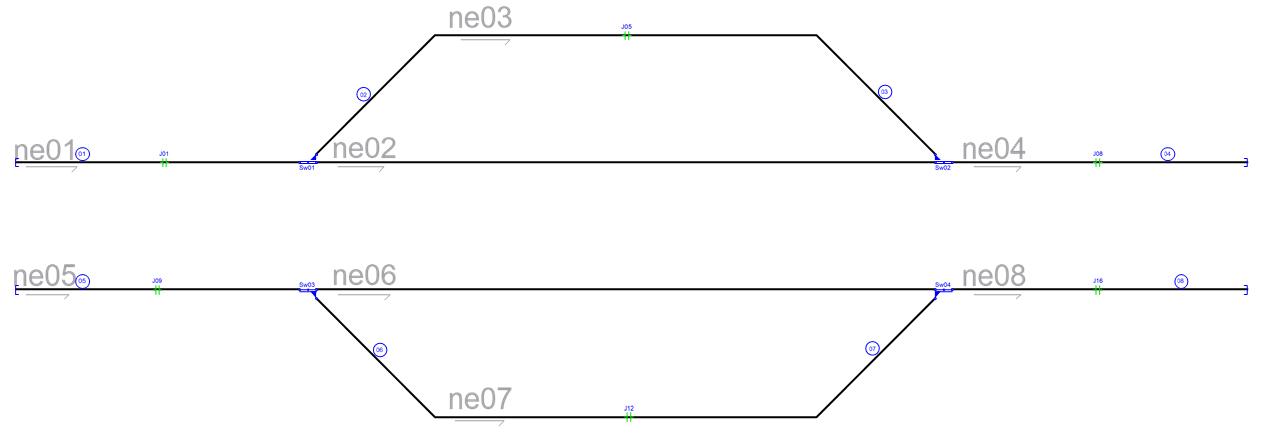
\includegraphics[width=1\textwidth]{resultados-obtenidos/ejemplo5/images/5_empty.png}
        \centering\caption{Topología ferroviaria del ejemplo 5 sin señalamiento.}
        %\label{fig:LC_P2}
    \end{figure}

    \begin{figure}[h]
        \centering
        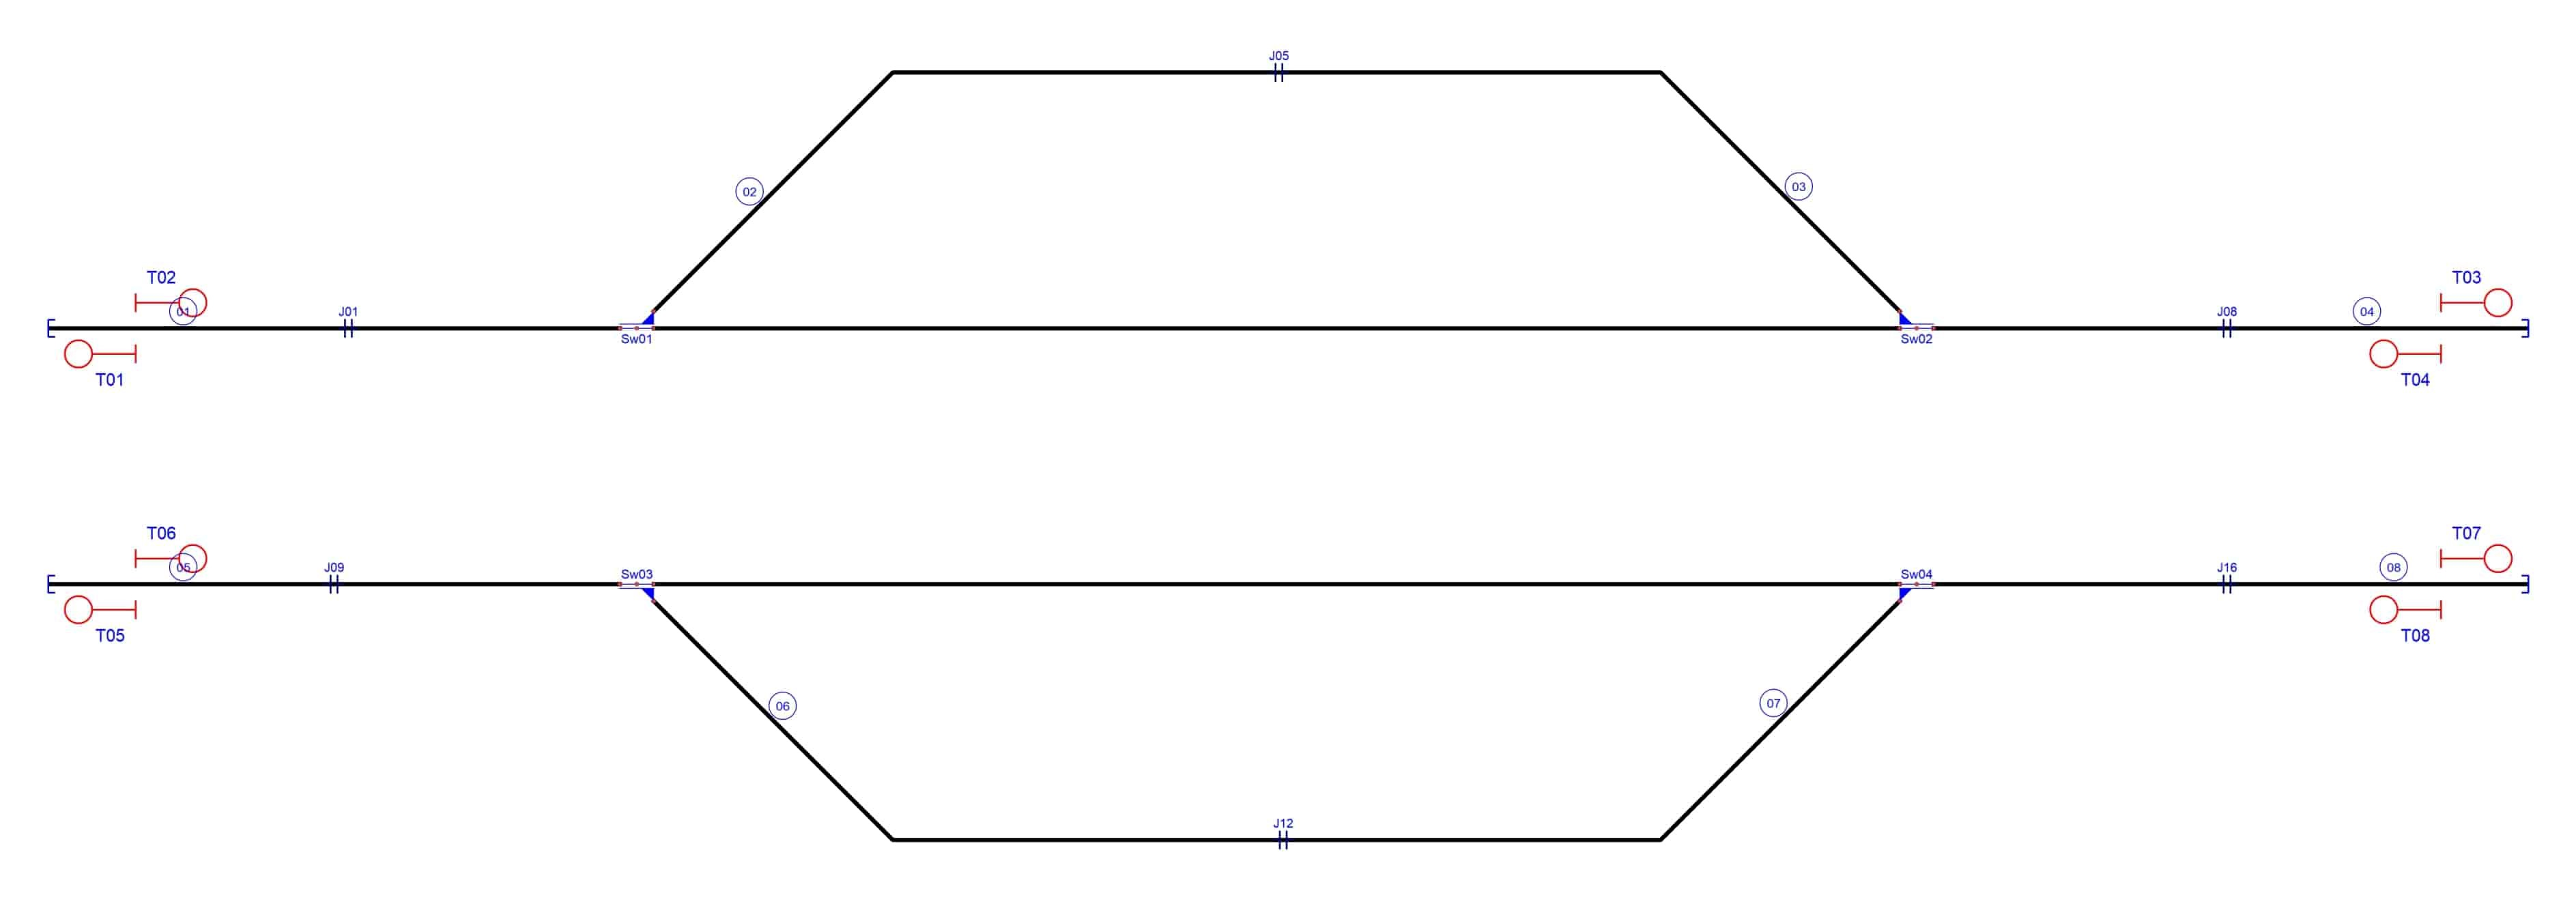
\includegraphics[width=1\textwidth]{resultados-obtenidos/ejemplo5/images/5_step1.png}
        \centering\caption{Señalamiento generado por el RNA para proteger el fín de vía.}
        %\label{fig:LC_P2}
    \end{figure}

    \begin{figure}[h]
        \centering
        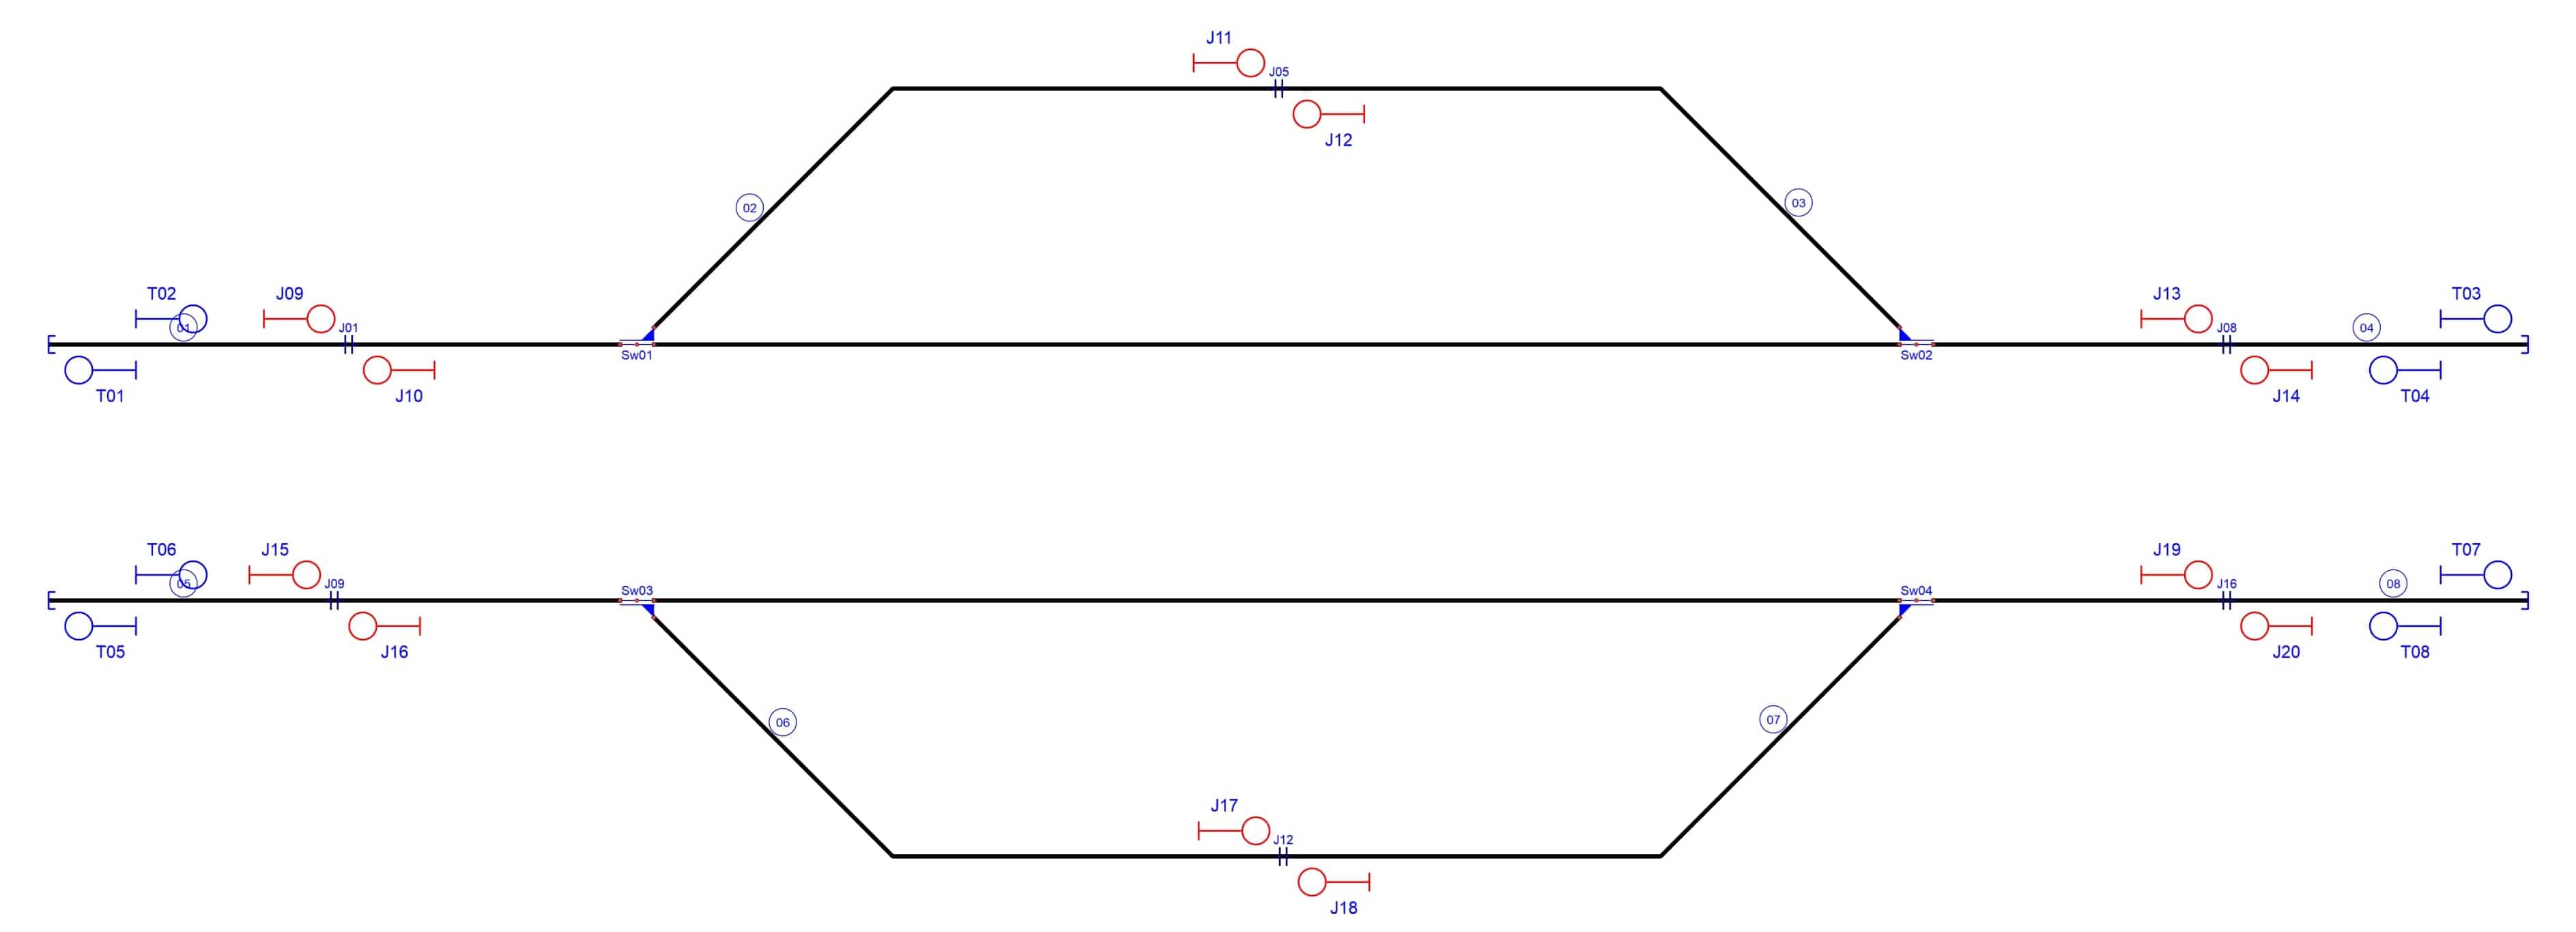
\includegraphics[width=1\textwidth]{resultados-obtenidos/ejemplo5/images/5_step2.png}
        \centering\caption{Señalamiento generado por el RNA para proteger las junturas.}
        %\label{fig:LC_P2}
    \end{figure}

    \begin{figure}[h]
        \centering
        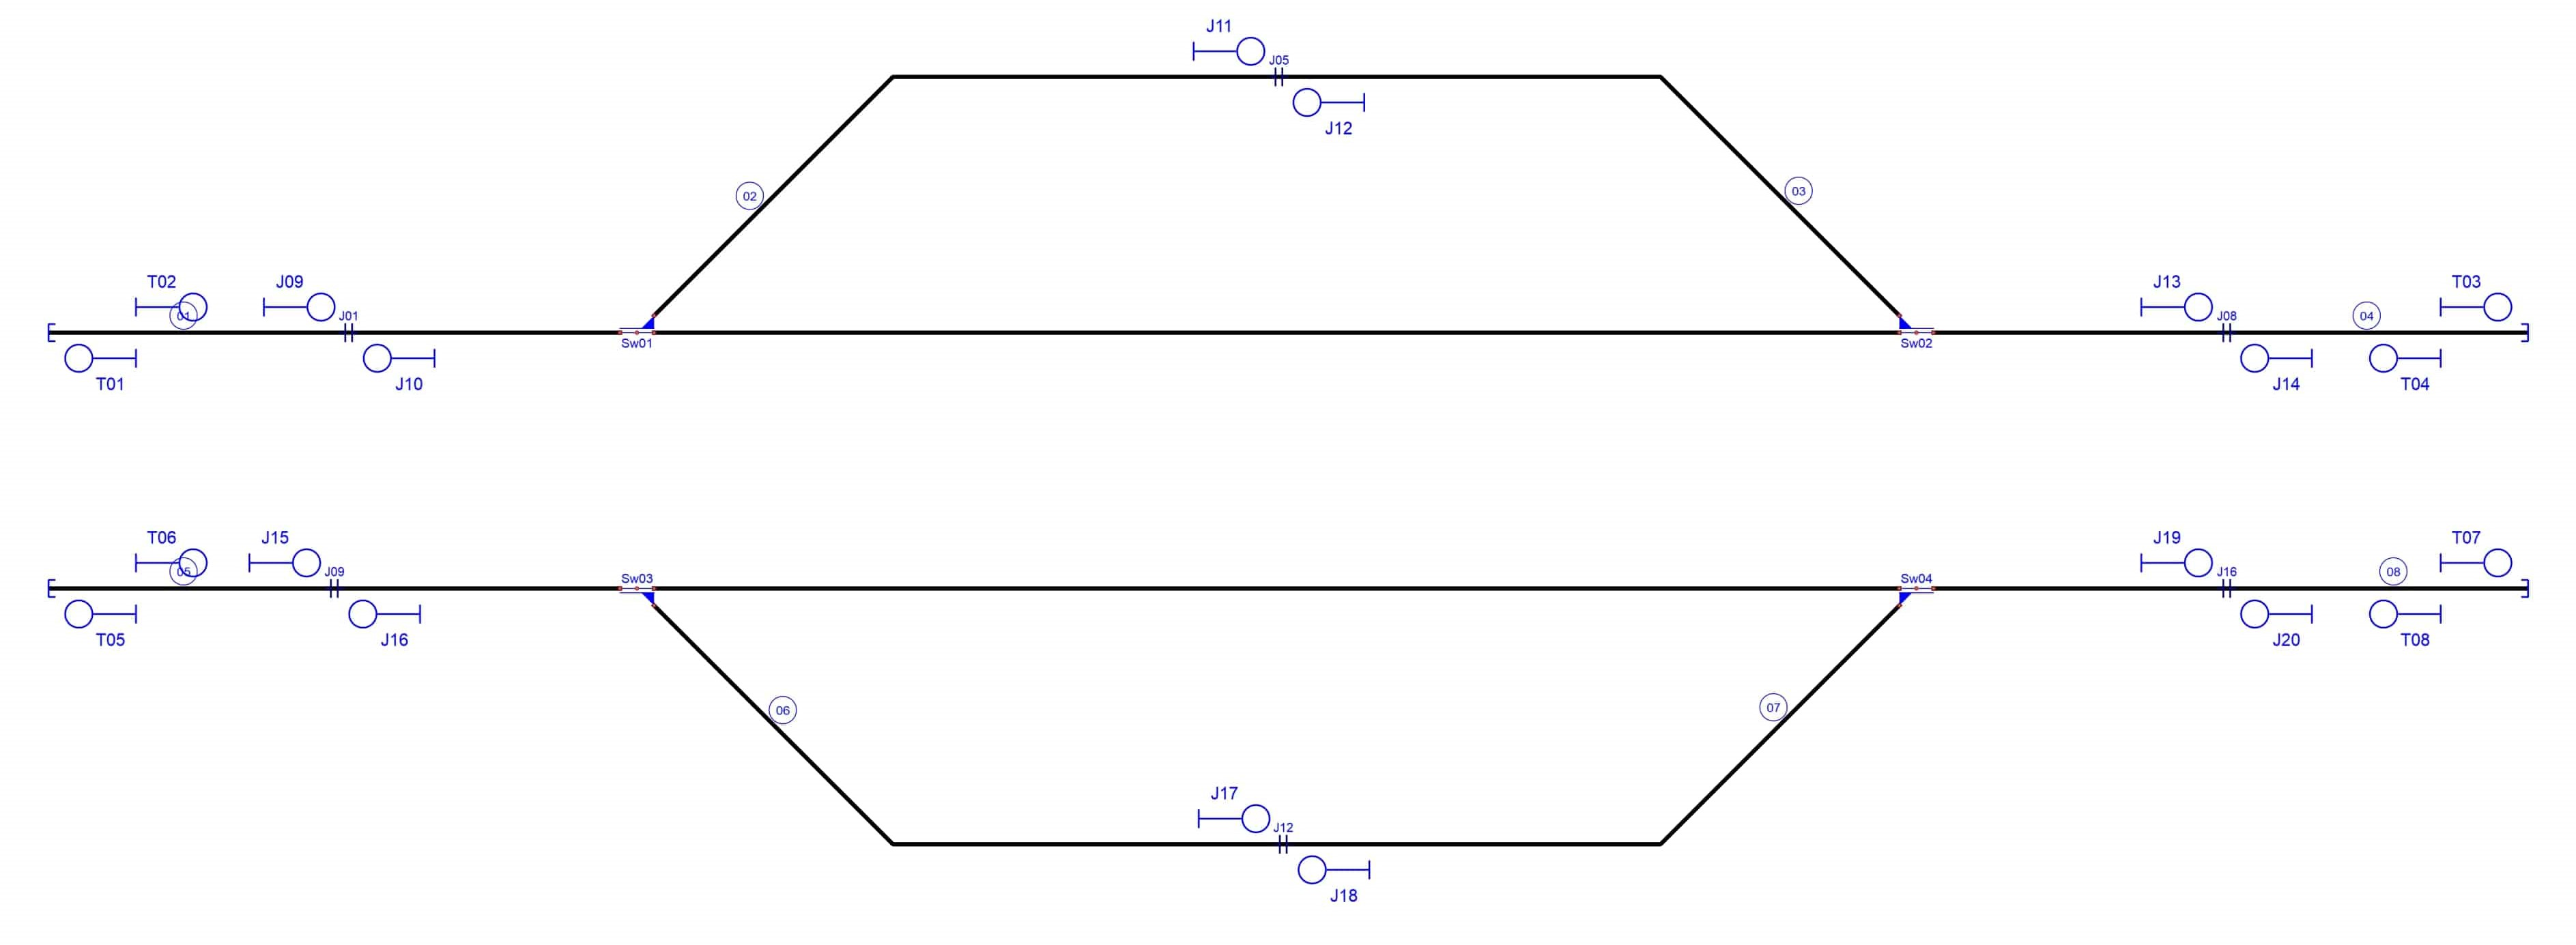
\includegraphics[width=1\textwidth]{resultados-obtenidos/ejemplo5/images/5_step3.png}
        \centering\caption{Señalamiento generado por el RNA para proteger plataformas y cruces de vía.}
        %\label{fig:LC_P2}
    \end{figure}

    \begin{figure}[h]
        \centering
        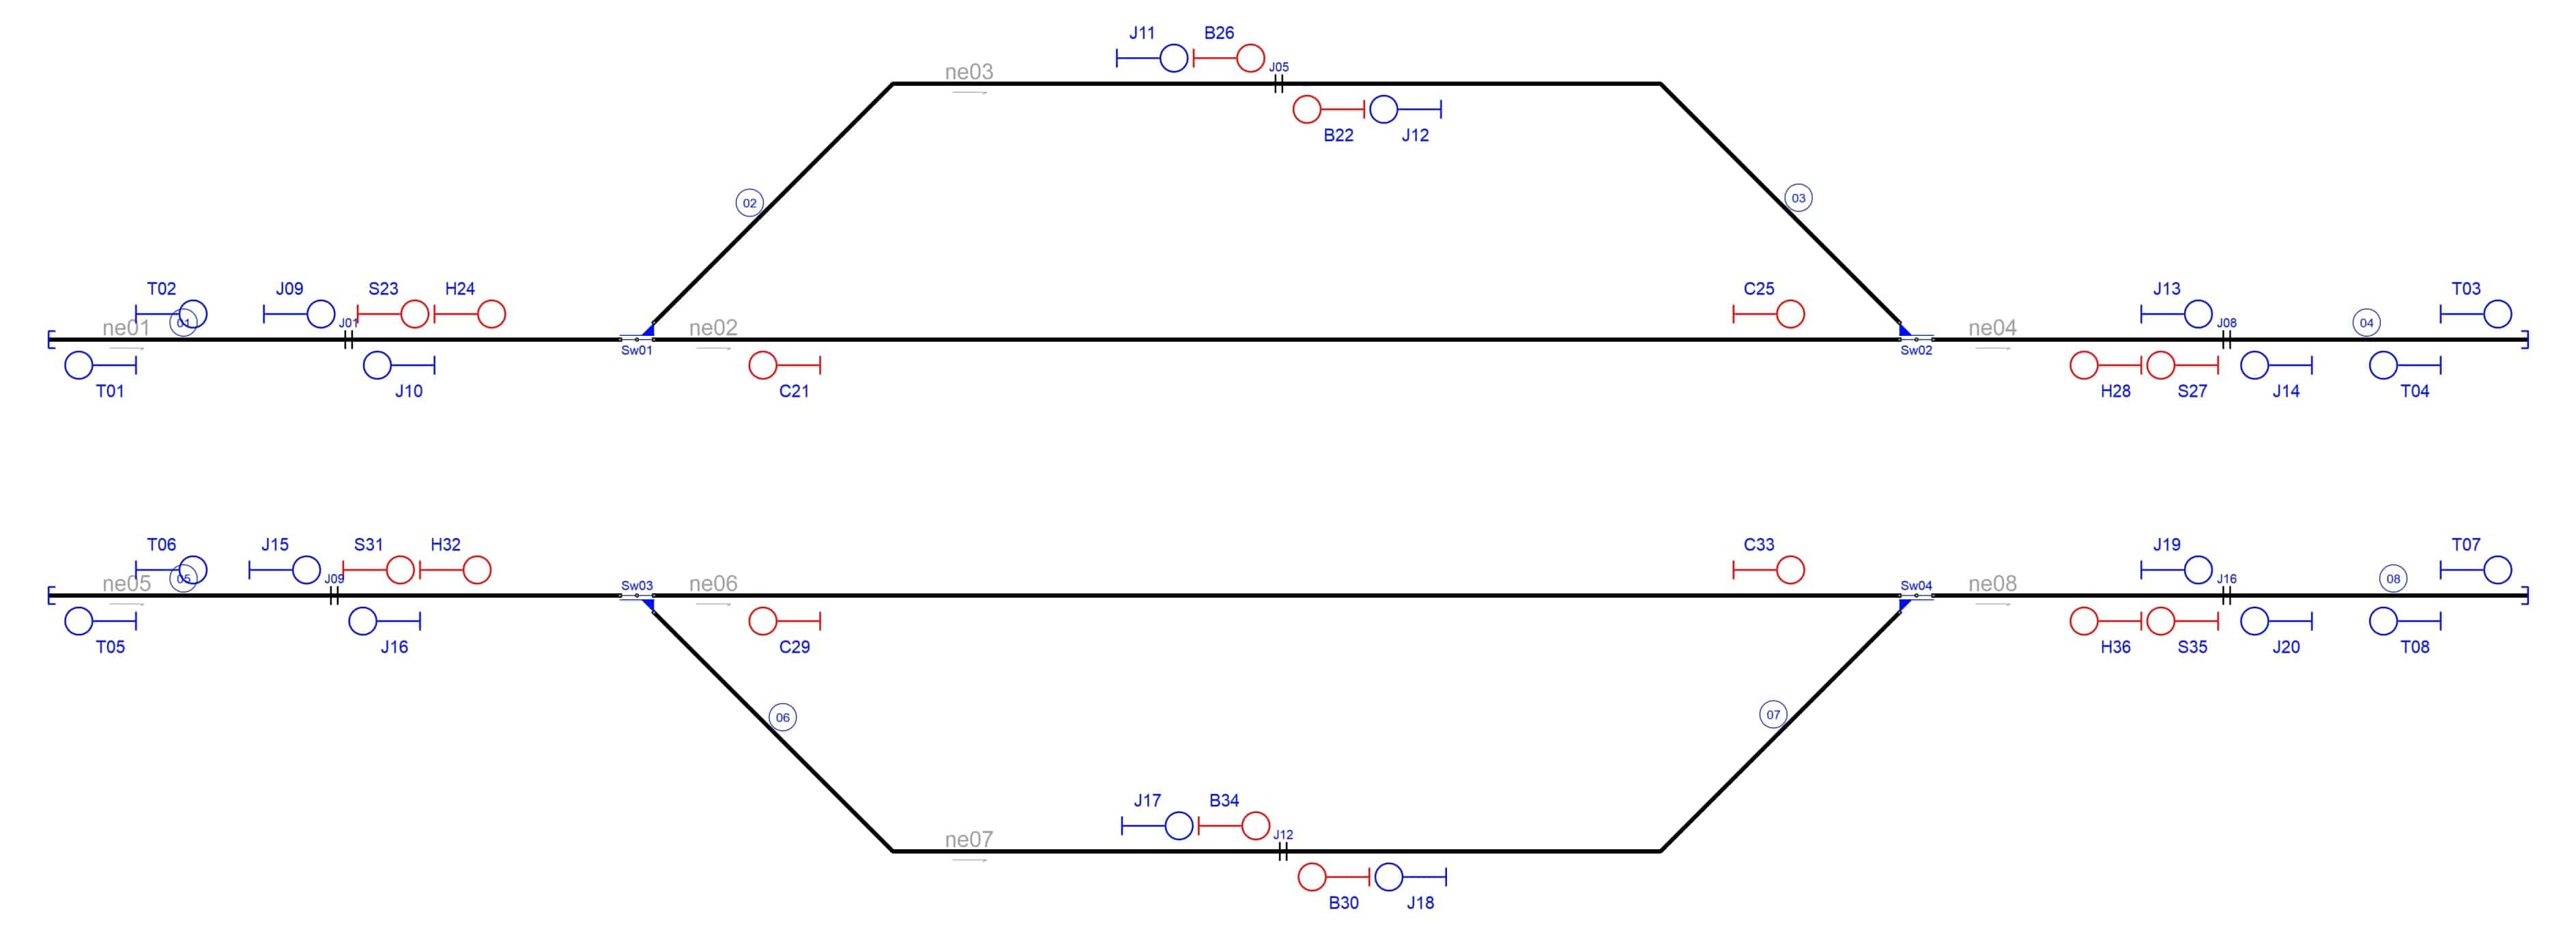
\includegraphics[width=1\textwidth]{resultados-obtenidos/ejemplo5/images/5_step4.png}
        \centering\caption{Señalamiento generado por el RNA para proteger las máquinas de cambios.}
        %\label{fig:LC_P2}
    \end{figure}

    \begin{figure}[h]
        \centering
        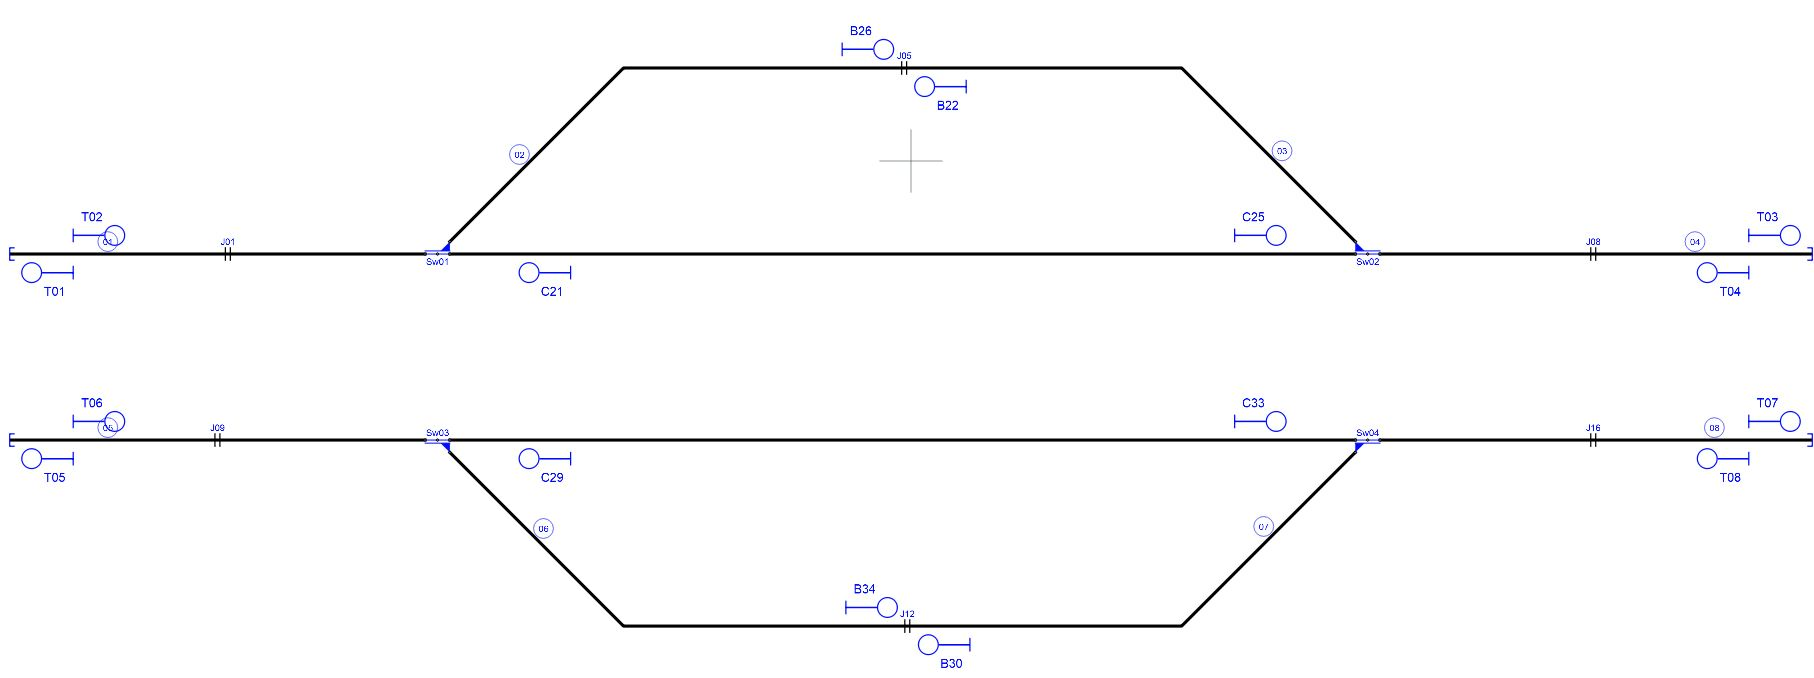
\includegraphics[width=1\textwidth]{resultados-obtenidos/ejemplo5/images/5_RNA.png}
        \centering\caption{Señalamiento generado y simplificado por el RNA.}
        %\label{fig:LC_P2}
    \end{figure}
    
    \subsection{Señalamiento original}

    \lipsum[1]
    
    \begin{table}[!h]
        {
        \caption{Tabla de enclavamiento original del ejemplo 5.}
        \label{Tab:tabla_original_5}
        \centering
        \resizebox{1\textwidth}{!}{
            \begin{tabular}{ c c c c c c c }
                \hline	
                    Ruta & Inicio & Final & Cambio & Plataforma & Cruce & netElement \\	
                \hline
                    R$_{01}$  & S$_{01}$ & S$_{06}$ & Sw$_{01}^{N}$ & - & - & ne$_{01}$-ne$_{02}$\\
                    R$_{02}$  & S$_{05}$ & S$_{13}$ & Sw$_{01}^{N}$ & - & - & ne$_{02}$-ne$_{01}$\\
                    R$_{03}$  & S$_{01}$ & S$_{03}$ & Sw$_{01}^{R}$ & - & - & ne$_{01}$-ne$_{03}$\\
                    R$_{04}$  & S$_{04}$ & S$_{13}$ & Sw$_{01}^{R}$ & - & - & ne$_{03}$-ne$_{01}$\\
                    R$_{05}$  & S$_{02}$ & S$_{04}$ & Sw$_{02}^{R}$ & - & - & ne$_{04}$-ne$_{02}$\\
                    R$_{06}$  & S$_{06}$ & S$_{15}$ & Sw$_{02}^{N}$ & - & - & ne$_{02}$-ne$_{04}$\\
                    R$_{07}$  & S$_{02}$ & S$_{05}$ & Sw$_{02}^{N}$ & - & - & ne$_{04}$-ne$_{03}$\\
                    R$_{08}$  & S$_{03}$ & S$_{15}$ & Sw$_{02}^{R}$ & - & - & ne$_{03}$-ne$_{04}$\\
                    R$_{09}$  & S$_{07}$ & S$_{11}$ & Sw$_{03}^{N}$ & - & - & ne$_{05}$-ne$_{06}$\\
                    R$_{10}$  & S$_{10}$ & S$_{14}$ & Sw$_{03}^{N}$ & - & - & ne$_{06}$-ne$_{05}$\\
                    R$_{11}$  & S$_{07}$ & S$_{09}$ & Sw$_{03}^{R}$ & - & - & ne$_{05}$-ne$_{07}$\\
                    R$_{12}$  & S$_{08}$ & S$_{14}$ & Sw$_{03}^{R}$ & - & - & ne$_{07}$-ne$_{05}$\\
                    R$_{13}$  & S$_{12}$ & S$_{10}$ & Sw$_{04}^{N}$ & - & - & ne$_{08}$-ne$_{06}$\\
                    R$_{14}$  & S$_{11}$ & S$_{16}$ & Sw$_{04}^{N}$ & - & - & ne$_{06}$-ne$_{08}$\\
                    R$_{15}$  & S$_{12}$ & S$_{08}$ & Sw$_{04}^{R}$ & - & - & ne$_{08}$-ne$_{07}$\\
                    R$_{16}$  & S$_{09}$ & S$_{16}$ & Sw$_{04}^{R}$ & - & - & ne$_{07}$-ne$_{08}$\\
                \hline
            \end{tabular}
        }
     }
    \end{table}
    \subsection{Señalamiento generado por el RNA}

    El RNA también exporta la misma información mostrada en el Código \ref{lst:EJ5_8} en una hoja de cálculo, similar a la que se visualiza en la Tabla \ref{Tab:tabla_generated_5}.
    
    \begin{table}[!h]
        {
        \caption{Tabla de enclavamiento del ejemplo 5 generada por el RNA.}
        \label{Tab:tabla_generated_5}
        \centering
        \resizebox{1\textwidth}{!}{
            \begin{tabular}{ c c c c c c c }
                \hline	
                    Ruta & Inicio & Final & Cambio & Plataforma & Cruce & netElement \\	
                \hline
                    R$_{01}$  & T$_{02}$ & C$_{25}$ & Sw$_{01}^{N}$ & - & - & ne$_{01}$-ne$_{03}$\\
                    R$_{02}$  & T$_{02}$ & B$_{26}$ & Sw$_{01}^{R}$ & - & - & ne$_{01}$-ne$_{04}$\\
                    R$_{03}$  & T$_{04}$ & C$_{21}$ & Sw$_{02}^{N}$ & - & - & ne$_{04}$-ne$_{03}$\\
                    R$_{04}$  & T$_{04}$ & B$_{26}$ & Sw$_{02}^{R}$ & - & - & ne$_{04}$-ne$_{04}$\\
                    R$_{05}$  & T$_{06}$ & C$_{33}$ & Sw$_{03}^{N}$ & - & - & ne$_{05}$-ne$_{06}$\\
                    R$_{06}$  & T$_{06}$ & B$_{34}$ & Sw$_{03}^{R}$ & - & - & ne$_{05}$-ne$_{07}$\\
                    R$_{07}$  & T$_{08}$ & C$_{29}$ & Sw$_{04}^{N}$ & - & - & ne$_{08}$-ne$_{06}$\\
                    R$_{08}$  & T$_{08}$ & B$_{30}$ & Sw$_{04}^{R}$ & - & - & ne$_{08}$-ne$_{07}$\\
                    R$_{09}$  & C$_{21}$ & T$_{01}$ & Sw$_{01}^{N}$ & - & - & ne$_{02}$-ne$_{01}$\\
                    R$_{10}$  & B$_{22}$ & T$_{01}$ & Sw$_{01}^{R}$ & - & - & ne$_{03}$-ne$_{01}$\\
                    R$_{11}$  & C$_{25}$ & T$_{03}$ & Sw$_{02}^{N}$ & - & - & ne$_{02}$-ne$_{04}$\\
                    R$_{12}$  & B$_{26}$ & T$_{03}$ & Sw$_{02}^{R}$ & - & - & ne$_{03}$-ne$_{04}$\\
                    R$_{13}$  & C$_{29}$ & T$_{05}$ & Sw$_{03}^{N}$ & - & - & ne$_{06}$-ne$_{05}$\\
                    R$_{14}$  & B$_{30}$ & T$_{05}$ & Sw$_{03}^{R}$ & - & - & ne$_{07}$-ne$_{05}$\\
                    R$_{15}$  & C$_{33}$ & T$_{07}$ & Sw$_{04}^{N}$ & - & - & ne$_{06}$-ne$_{08}$\\
                    R$_{16}$  & B$_{34}$ & T$_{07}$ & Sw$_{04}^{R}$ & - & - & ne$_{07}$-ne$_{08}$\\
                \hline
            \end{tabular}
        }
     }
    \end{table}
    
    En una primera inspección podemos ver que el nuevo señalamiento tiene 16 rutas, al igual que el señalamiento original que también posee 16 rutas. Esto se debe a que el señalamiento original ya contemplaba todas las rutas posibles y el RNA generó un nuevo señalamiento equivalente, sin eliminar rutas ni tampoco agregando rutas que no sean útiles.
    \section{Sistema generado por el ACG}

	En base a la red de grafos, ilustrada en la Figura \ref{fig:EJ5_8}, el ACG determinó la siguiente cantidad de elementos, tal puede visualizarse en el Código \ref{lst:EJ5_8}.
	
	\begin{lstlisting}[language = {}, caption = Cantidad de elementos a implementar por el ACG, label = {lst:EJ5_8}]
	n_netElements:8
	n_switch:4
	n_doubleSwitch:0
	n_borders:0
	n_buffers:4
	n_levelCrossings:0
	n_platforms:0
	n_scissorCrossings:0
	n_signals:16
	N : 44
	\end{lstlisting}
	
	Se repetirán los pasos detallados en el ejemplo 1, Sección \ref{sec:EJEMPLO1_ACG}, por lo que solamente se destacarán aspectos particulares de este ejemplo. El ACG genera 62 archivos en formato VHDL. El archivo \textit{Arty\_Z7-10.XDC} es el mismo para todos los ejemplos, al ser invariante respecto a la cantidad de pines a utilizar. Se deberá modificar el script mostrado en el Código \ref{lst:EJ1_script} y cambiar el parámetro \textit{chosen} a 5 para automatizar la importación de los archivos del ejemplo 5 y desvincular cualquier otro conjunto de archivos de ejemplos anteriores.
	
	Una vez ejecutado el script, Vivado ordenará los archivos de forma jerárquica, donde el módulo \textit{global} incluye todos los módulos que fueron detallados en la Sección \ref{sec:interlockingArch}. Cada una de las instancias del módulo \textit{network} contienen sus propias 44 instancias de los mismos módulos de cada elemento ferroviario ya que N, cantidad de elementos ferroviarios, es 44 en el Código \ref{lst:EJ5_8}. El ejemplo 5 utiliza mas de 13800 sub módulos conectados automáticamente mediante mas de 27000 señales, lo cual se aleja bastante de un desarrollo que pueda realizarse manualmente de forma trivial.
	
	Cuando Vivado genera el diagrama de bloques ya tenemos la certeza de que el código VHDL ha pasado la prueba de sintaxis del entorno de desarrollo. A continuación, se deberá sintetizar e implementar el sistema para generar el bitstream que será utilizado para programar la FPGA. Los procesos de síntesis e implementación fueron detallados en el ejemplo 1, Sección \ref{sec:EJEMPLO1_ACG}.
	
	Los resultados de ambos procesos son detallados en la Tabla \ref{Tab:tabla_ACG_5}. Los porcentajes de uso son calculados por Vivado automáticamente, teniendo en cuenta que la plataforma Arty Z7 20 posee 53200 Look-Up-Tables (LUTs), 106400 Flip-Flops (FFs), 125 Pines de entrada y salida (IOs) y 32 Buffers (BUFGs), tal cómo se explicó en la Sección \ref{sec:AGG}. En este ejemplo, la cantidad de recursos utilizados es baja y el tiempo de síntesis e implementación es de 41 y 57 segundos, respectivamente.
		
	\begin{table}[H]
		{
			\caption{Síntesis e implementación del ejemplo 5 generado por el ACG.}
			\label{Tab:tabla_ACG_5}
			\centering
			%\small
			%\centering
			\begin{center}
				\resizebox{0.7\textwidth}{!}{
					\begin{tabular}{ c c c c }
						\hline	
						Recursos & Síntesis & Implementación & Uso \\	
						\hline
						LUT & 2328 & 2307 & 4.38-4.34\%\\
						FF & 2344 & 2347 & 2.20-2.21\%\\
						IO & 15 & 15 & 12.00\%\\
						BUFG & 3 & 3 & 9.38\%\\
						\hline
					\end{tabular}
				}
			\end{center}
		}    
	\end{table}
    \section{Validación del sistema}

    La validación de las rutas de la tabla de enclavamientos es realizada por el RNA aplicando el Algoritmo \ref{alg:interlocking_tables}, explicado en la Sección \ref{sec:validar_tabla}. Las 16 rutas del señalamiento original (Tabla \ref{Tab:tabla_original_5}) tienen 16 rutas equivalentes en el señalamiento generado por el RNA (Tabla \ref{Tab:tabla_generated_5}), tal como se puede visualizar en la Tabla \ref{Tab:tabla_validation_5}, generada automáticamente por el RNA.

    \begin{table}[!h]
        {
        \caption{Equivalencias entre las rutas originales y las generadas por el RNA.}
        \label{Tab:tabla_validation_5}
        \centering
        \resizebox{0.9\textwidth}{!}{
            \begin{tabular}{ c c c c }
                \hline	
                    Original & Señales & RNA & Señales \\	
                \hline
                    R$_{01}$ & S$_{01}$-S$_{06}$ & R$_{01}$ & T$_{02}$-C$_{25}$ \\
                    R$_{02}$ & S$_{05}$-S$_{13}$ & R$_{09}$ & C$_{21}$-T$_{01}$ \\
                    R$_{03}$ & S$_{01}$-S$_{03}$ & R$_{02}$ & T$_{02}$-B$_{26}$ \\
                    R$_{04}$ & S$_{04}$-S$_{13}$ & R$_{10}$ & B$_{22}$-T$_{01}$ \\
                    R$_{05}$ & S$_{02}$-S$_{04}$ & R$_{03}$ & T$_{04}$-C$_{21}$ \\
                    R$_{06}$ & S$_{06}$-S$_{15}$ & R$_{11}$ & C$_{25}$-T$_{03}$ \\
                    R$_{07}$ & S$_{02}$-S$_{05}$ & R$_{04}$ & T$_{04}$-B$_{26}$ \\
                    R$_{08}$ & S$_{03}$-S$_{15}$ & R$_{12}$ & B$_{26}$-T$_{03}$ \\
                    R$_{09}$ & S$_{07}$-S$_{11}$ & R$_{05}$ & T$_{06}$-C$_{33}$ \\
                    R$_{10}$ & S$_{10}$-S$_{14}$ & R$_{13}$ & C$_{29}$-T$_{05}$ \\
                    R$_{11}$ & S$_{07}$-S$_{09}$ & R$_{06}$ & T$_{06}$-B$_{34}$ \\
                    R$_{12}$ & S$_{08}$-S$_{14}$ & R$_{14}$ & B$_{30}$-T$_{05}$ \\
                    R$_{13}$ & S$_{12}$-S$_{10}$ & R$_{07}$ & T$_{08}$-C$_{29}$ \\
                    R$_{14}$ & S$_{11}$-S$_{16}$ & R$_{15}$ & C$_{33}$-T$_{07}$ \\
                    R$_{15}$ & S$_{12}$-S$_{08}$ & R$_{08}$ & T$_{08}$-B$_{30}$ \\
                    R$_{16}$ & S$_{09}$-S$_{16}$ & R$_{16}$ & B$_{34}$-T$_{07}$ \\
                \hline
            \end{tabular}
     		}
        }    
    \end{table}
    
    Todas las rutas generadas por el RNA (Tabla \ref{Tab:tabla_generated_5}) tienen una ruta equivalente en el señalamiento original (Tabla \ref{Tab:tabla_original_5}). El RNA no ha generado nuevas señales ni rutas ya que el señalamiento original ya satisfacía todos los requerimientos de seguridad necesarios. Tampoco se eliminaron señales ni rutas, lo que demuestra que el RNA puede mejorar los sistemas de enclavamientos cuando es posible, o igualarlos cuando se ha alcanzado la cota máxima de seguridad, sin recurrir a redundancias improductivas.
    
    Para finalizar, el RNA comprueba los principios de señalamiento ferroviario explicados en la Sección \label{sec:validar_principios}, aplicando los algoritmos indicados, de los cuáles se obtuvieron los siguientes resultados:
    
    \begin{itemize}
    	\item Principio de autoridad (Algoritmo \ref{alg:ppio_autoridad}): cobertura del 100\% de los \textit{netElements}.
    	\item Principio de claridad (Algoritmo \ref{alg:ppio_claridad}): rutas 100\% independientes.
    	\item Principio de anticipación (Algoritmo \ref{alg:ppio_anticipacion}): cobertura del 100\% de los puntos críticos.
    	\item Principio de granularidad (Algoritmo \ref{alg:ppio_granularidad}): 100\% de rutas divididas a su mínima expresión.
    	\item Principio de terminalidad (Algoritmo \ref{alg:ppio_terminalidad}): 100\% de finales de vías protegidos.
    	\item Principio de infraestructura (Algoritmo \ref{alg:ppio_infraestructura}): 100\% de infraestructura protegida.
    	\item Principio de no bloqueo (Algoritmo \ref{alg:ppio_nobloqueo}): 100\% de cambios de vías protegidos.
    \end{itemize}	